\subsection{3D Simulator}
\label{sec:sf-simulator}
\writer{Anders}

The 3D Simulator will show the animated Petri net, while allowing the user to control a few things. The functionality of the 3D simulator can be specified using the following statements.

\subsubsection{Functional Requirements}
\begin{enumerate}
\item The Simulator \textbf{shall} allow the user to play the simulation.
\item The Simulator \textbf{shall} allow the user to pause the simulation.
\item The Simulator \textbf{shall} allow the user to reset the simulation.
\item The Simulator \textbf{shall} allow the user to add tokens on input places.
\item The Simulator \textbf{shall} allow the user to exit the simulation.
\item The Simulator \textbf{should} allow the user to change the orientation of the view.
\item It \textbf{would be nice} if the Simulator allowed the user to take screenshots.
\item It \textbf{would be nice} if the Simulator allowed the user to forward the simulation.
\item It \textbf{would be nice} if the Simulator allowed the user to rewind the simulation.
\end{enumerate}

\subsubsection{Use cases}

The features described above are shown in Figure~\ref{fig:use-cases-simulator}.

\begin{figure}[htp]
\begin{center}
  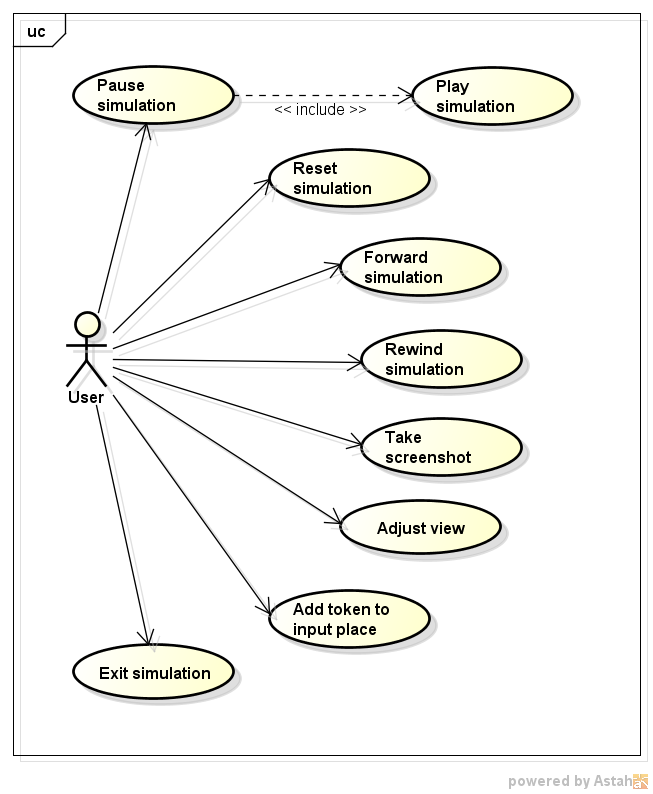
\includegraphics[width=0.5\textwidth]{image/uc-simulator.png}
  \caption{Use cases for the 3D Simulator}
  \label{fig:use-cases-simulator}
\end{center}
\end{figure}